\section{Methodology} \label{ch6:studysettings}

In this study, we perform both qualitative and quantitative analyses with
respect to the delivery delay phenomena. We gather our data by surveying and
interviewing the team members (\ie participants) of our subject projects. In
this section, we describe the subject projects and how we collect and analyze
our data.

\subsection{Subjects}

We surveyed 37 participants of the Firefox, ArgoUML, and Eclipse (JDT) projects.
We naturally choose these projects, since the analyses of this study is intended
to complement our prior quantitative analyses that we performed in those
projects.  We provide a brief description of each subject project below (we have
already provided a detailed description in
\hyperref[ch4:sec:subjects]{Section}~\ref{ch4:sec:subjects}).

ArgoUML is an open source UML modeling tool. ArgoUML provides support for all of
the UML 1.4 diagrams. At the time that we perform this study, ArgoUML was
downloaded 80,000 times worldwide.\smartfoot{\url{http://argouml.tigris.org}}
ArgoUML uses the IssueZilla ITS to record its issue
reports.\smartfoot{\url{http://argouml.tigris.org/project_bugs.html}}

Eclipse is a popular {\em Integrated Development Environment} (IDE) that is
famous for its support for the Java programming
language.\smartfoot{\url{https://eclipse.org/}} We study the {\em Java
Development Tools} (JDT) project of the Eclipse
Foundation.\smartfoot{\url{https://projects.eclipse.org/projects/eclipse.jdt}}
The JDT project provides the Java perspective for the Eclipse IDE, which
includes a number of views, editors, wizards, and builders. 

ArgoUML and Eclipse (JDT) adopt a traditional release cycle when compared to the
Firefox project. For instance, the median duration of release cycles that we
study for the ArgoUML and Eclipse (JDT) projects are 180 and 112 days,
respectively (see \hyperref[ch:study12]{Chapter}~\ref{ch:study12}). While we are
able to study the perceived impact of adopting rapid releases when surveying the
participants of the Firefox project, we ask the participants of the other
projects to conjecture how such an impact would be (\ie the impact on delivery
delays). 

\subsection{Data collection}\label{ch5:datacollection2}

\begin{table}[t!]
	\centering
	\footnotesize
	\caption{\textbf{Survey questions (excerpt).} Each horizontal line indicates a page break.
	\label{tbl:survey}}
		\begin{tabular}{p{0.95\textwidth}}
			\hline 
			\textbf{1.} For how long have you been developing software? {\em (dropdown)}\tabularnewline
			\textbf{2.} For how long have you worked in the (Firefox/ArgoUML/Eclipse) project?
			{\em (dropdown)}\tabularnewline
			\textbf{3.} How would you describe your roles in the software development of
			the Firefox/ArgoUML/Eclipse project? (e.g., developer, tester, release manager, etc.)
			{\em (text box)}\tabularnewline
			\textbf{4.} In your opinion, what motivates a development team to shift from
			a traditional release cycle (e.g., a release every 9 to 18 months)
			to a rapid release cycle (e.g., a release every 6
			weeks)? {\em (text box)}\tabularnewline
			\textbf{5.} In this survey, we consider that an issue is completed when it
			is implemented and tested, i.e., it is ready to be delivered. Do
			you remember an issue that the development team completed work on,
			but was not delivered to end users through the next possible release?
			Can you tell us what caused the delivery delay of this issue in your
			opinion? {\em (text box)}\tabularnewline
			\textbf{6.} In your experience, how common are the cases in which completed
			issues (issues that are implemented and tested) are omitted from the
			next possible release?\tabularnewline
			\textbf{7.} Who decides when a completed issue is delivered into an official
			release in your team? {\em (text box)}\tabularnewline
			\textbf{8.} In your opinion, when is the delivery of a completed issue to the
			end user considered to be delayed in your project? {\em (text box)}\tabularnewline
			\hline 
			\textbf{9.} In your opinion, is it frustrating to users when a completed issue
			skips one or more releases? Why? {\em (text box)}\tabularnewline
			\textbf{10.} Is it frustrating for the team members when a completed issue
			skips one or more releases? Why? {\em (text box)}\tabularnewline
			\hline 
			\textbf{11.} Assuming that an issue is completed today (implementation and
			testing are completed), what reasons can you think of for the issue
			not to be delivered to end users in the next release? {\em (text box)}\tabularnewline
			\hline 
			\textbf{12.} What can team members do to avoid the delivery delay of completed
			issues? {\em (text box)}\tabularnewline
			\textbf{13.} To what extent do you agree that the characteristics listed in
			the table below are related to the delivery delay of a
			completed issue?\\
			- The reporter of an addressed issue, the resolver of an
			addressed issue, the priority level, the severity level,
			number of comments, number of modified files, number of
			lines of code, the time at which an issue was addressed
			during the release cycle.
			{\em (5-point Likert scale for each option)}\tabularnewline
			\hline 
			\textbf{14-Firefox.} Have you worked in both traditional and rapid release cycles of
			the Firefox project? {\em (yes/no)}\tabularnewline
			\textbf{15-Firefox.} In your opinion, how much impact does a rapid release cycle have
			on the time to deliver completed issues for end users?
			{\em (text box)}\tabularnewline
			\textbf{16-Firefox.} Did your project evaluate the shift to rapid release cycles? If
			so, how? {\em (text box)}\tabularnewline
			\textbf{14-Others.} Do you have experience working on a
			rapid release cycle in any other project? {\em (yes/no)}\tabularnewline
			\textbf{15-Others.} In your opinion, what would be the
			impact of shifting to a rapid release cycle (e.g., a
			release every 6 weeks rather than a release every 9 to
			18 months) on the delay to deliver completed issues, in
			your project? {\em (text box)}\tabularnewline
			\textbf{16-Others.} If your project had shifted from a
			traditional to a rapid release cycle, how would you
			evaluate if this shift benefited your project? {\em (text box)}
		\end{tabular}
\end{table}

To collect the data to perform our third study, we design a web-based survey
that was sent to 780 participants of the Firefox, Eclipse (JDT), and ArgoUML
projects. Before sending our survey to the participants of the studied projects,
we sent a pilot survey to 10 participants of two distinct brazilian software
development companies. After receiving the answers, we improved our questions to
better reflect what we intended to understand from our participants.

We sent our polished survey to 513 Firefox, 184 Eclipse (JDT), and 83 ArgoUML
participants. We gathered the participants' e-mails from the respective
developer mailing list archives of each studied project. We consider e-mail
addresses from messages that were sent in the past 4 years. To encourage
participation, we provided \$100 Amazon.com gift cards to a random subset of the
respondents who answered all of the questions of our surveys.

Our survey is based on the two major {\em themes} that are investigated in this
thesis. The first {\em theme} is about
delivery delay in general, while the second {\em theme} is focused on the
impact of switching to a rapid release cycle on the delivery delay (see
\hyperref[fig:thesis_overview]{Figure}~\ref{fig:thesis_overview}). In
particular, we are interested on understanding the perceived advantages and disadvantages of
adopting rapid releases with respect to delivery delays. In
\hyperref[tbl:survey]{Table}~\ref{tbl:survey}, we highlight a subset of the
questions of our survey. Each horizontal line represents a page break in the
survey. Our complete surveys are available in
\hyperref[appendix:a]{Appendices}~\ref{appendix:a},~\ref{appendix:b},~and~\ref{appendix:c}.
The first three questions collect demographic information. Questions \#5-13
belong to the general delivery delay {\em theme}, while questions \#4,
\#14-16 belong to the impact of switching to a rapid release cycle {\em theme}.
We placed one question of the second {\em theme} early in the survey to mitigate
bias in the responses about the motivation to switch to a rapid release cycle.
Finally, questions \#14-16 are different for the Firefox project, since the
other projects did not shift from a traditional to a rapid release cycle. 

In total, we receive 37 responses (5\% response rate), of which 25 responses
come from Firefox participants, 9 from Eclipse participants, and 3 from ArgoUML
participants. During our survey, we ask if the participant is willing to perform
a follow-up interview. In total, we perform 4 follow-up interviews (from
the 8 participants that declared to be willing to do so).  

The goal of our follow-up interviews is to gather deeper insights into the
responses of the participants. In particular, we intend to {\em (i)} better
understand the reasons as to why they assign a given rank to the factors that
are presented in {\em question \#13}, {\em (ii)} gather more details about why
do they agree or disagree with our quantitative data of prior studies, and {\em
(iii)} recover feedback when they do not answer a specific question or do not
understand it.  Our interviews are semi-structured (\ie we did not strictly
follow our script in case our interviewee provides more subjects to discuss).
For the interested reader, the invitation letter of our survey and the script
that guided our interviews are available at
\hyperref[invitation_letter]{Appendices}~\ref{invitation_letter}
and~\ref{interview_script}.

\subsection{Research Approach}

Given the geographic limitations to perform in-person meetings, the author of
this thesis and co-author~\#1 independently conduct three sessions of open
coding of the responses to open-ended questions (one session for each RQ). In
the following, the codes that were generated are shared and merged into a new
set of codes. The co-author~\#2 reviews the set of codes and adds additional
entries to the final set of codes. At the end of the process, we achieve 175
unique codes. Finally, we group our codes into higher-level conceptual {\em
themes} in order to answer our RQs. The codes that were produced during our open
coding sessions as well as our participants' responses are publicly available
online.\smartfoot{\url{http://danielcalencar.github.io/materials.html}}

\begin{table}
	\footnotesize
	\centering
	\caption{Participant range per subject project.
		\label{tbl:participants}
	}
	\begin{tabular}{lc}
		\hline 
		\textbf{Project} & \textbf{Participant range}\tabularnewline
		\hline 
		\hline 
		Firefox & F01--F25\tabularnewline
		\hline 
		Eclipse & E26--E34\tabularnewline
		\hline 
		ArgoUML & A35--A37\tabularnewline
		\hline 
	\end{tabular}
\end{table}

When reporting the results of \hyperref[ch5:rq1]{RQ1}-\hyperref[ch5:rq3]{RQ3},
we indicate in superscript the number of participants that mentioned a
particular code that emerged during the qualitative analysis. These numbers do
not necessarily indicate the importance of a given code, since they were coded
based on the received responses rather than scored by the participants. Also, we
mention quotes from the interviews when necessary to provide more detail about
the results. Finally, \hyperref[tbl:participants]{Table}~\ref{tbl:participants}
shows the IDs of the participants that we use while reporting results.

Finally, we also perform quantitative analyses of the responses to Likert-scale
questions. First, we check if the factors that are listed in {\em question~\#13}
are significantly different using the ranks (responses) that are assigned to
each factor. We use a Kruskal Wallis test~\cite{kruskal1952use} to check if
there is a statistically significant difference between the ranks assigned to
the factors. The Kruskal Wallis test is the non-parametric equivalent of the
ANOVA test~\cite{fisher1925statistical} to check if there are statistically
significant differences when comparing three or more distributions. Since
Kruskal Wallis does not indicate which factor has statistically different values
with respect to others, we use the Dunn test~\cite{dunn1964multiple} to perform
specific comparisons. For example, the Dunn test indicates whether the ranks
that are assigned to the {\em number of comments} metric are statistically
different when compared to the ones that are assigned to the {\em number of
modified files} metric. We use the Bonferroni correction~\cite{dunn1961multiple}
on the obtained $p$ values to account for the multiple comparisons that we
perform between each of the factors that are listed in {\em question~\#13}. 

Additionally, we correlate the ranks that are assigned to the factors in {\em
question~\#13} with the experience of the participants ({\em question~\#1}). To
do so, we use Spearman rank {$\rho$} correlation~\cite{spearman1904proof}, which
is used to measure the statistical dependence between the ranks of two
variables. Finally, we also correlate the experience of the participants with
the perception of the frequency of delivery delay that happens in the studied
projects ({\em question~\#6}).

\subsection{Demographics}\label{subsubsec:exploratory}

\begin{figure}
	\centering
	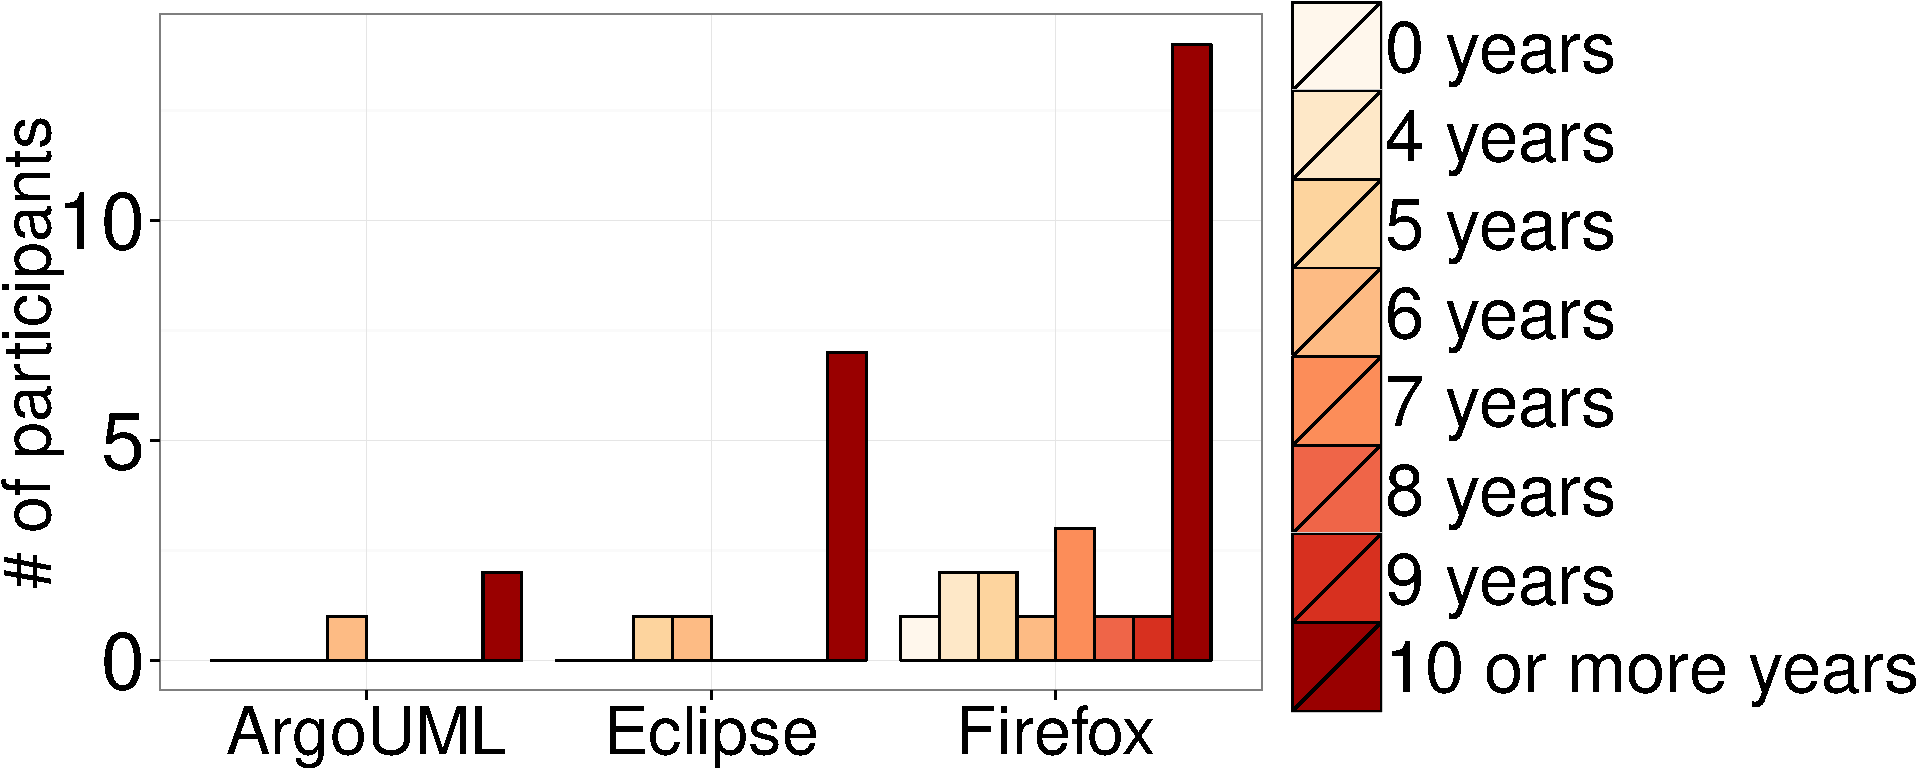
\includegraphics[width=0.80\textwidth,keepaspectratio] 
	{chapters/chapter5/figures/demographic_experience.pdf}
	\caption{Software development experience of the participants.}
	\label{fig:demographics_experience}
\end{figure}
We present the demographics of our obtained data.
\hyperref[fig:demographics_experience]{Figure}~\ref{fig:demographics_experience}
shows the experience of the participants. We collect this data from {\em
question~\#1}. The options range from ``0 years'' to ``10 or more years''. We
observe that 62\% ($\frac{23}{37}$) of the participants have ``10 or more
years'' of software development experience. 
\begin{figure}
	\centering
	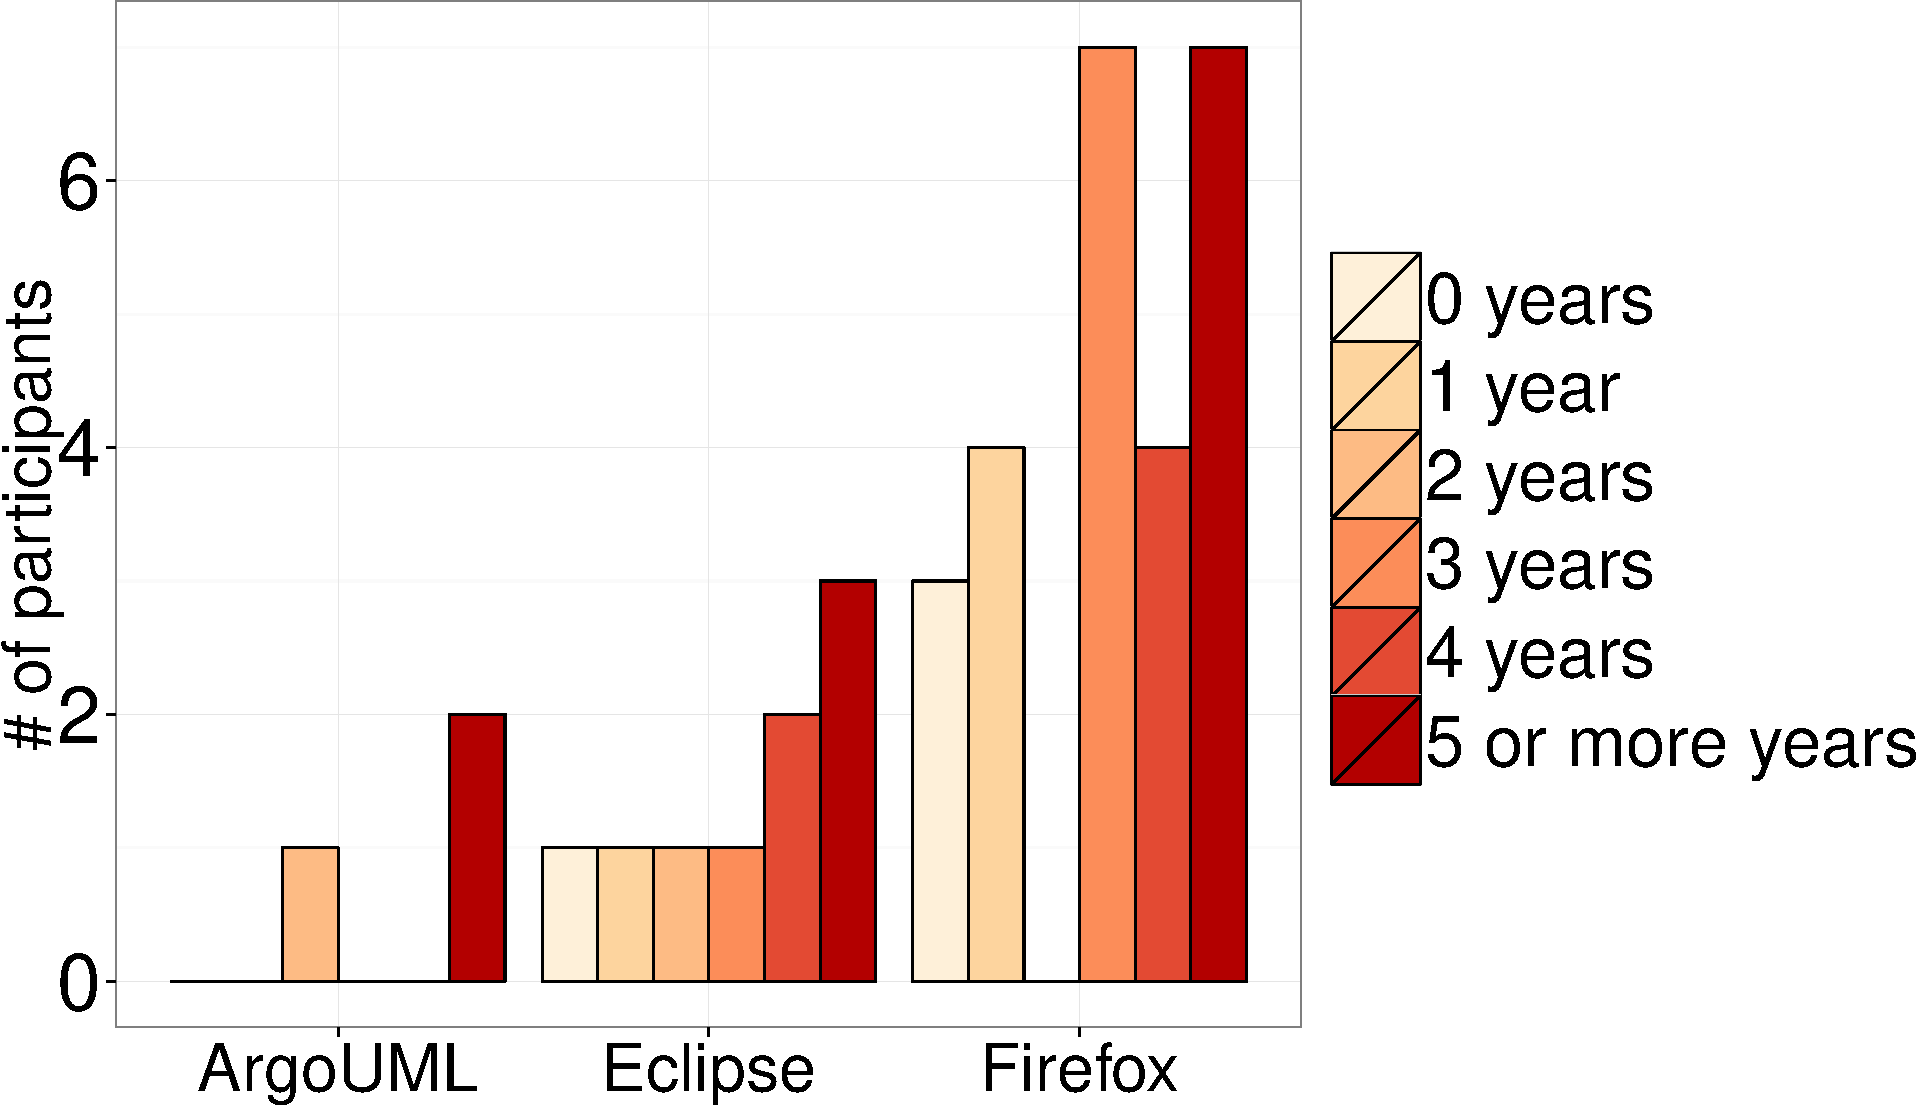
\includegraphics[width=0.80\textwidth,keepaspectratio] 
	{chapters/chapter5/figures/demographic_experience_project.pdf}
	\caption{Development experience of the participants in the
	respective project.}
	\label{fig:demographics_experience_project}
\end{figure}
Furthermore,
\hyperref[fig:demographics_experience_project]{Figure}~\ref{fig:demographics_experience_project}
shows the experience of the participants related to the specific project that
they are representing. We collect this data from {\em question~\#2} and the
options range from ``0 years'' to ``5 or more years''. 51\%  ($\frac{19}{37}$)
of the participants have 4 or more years of experience. 
\begin{figure}
	\centering
	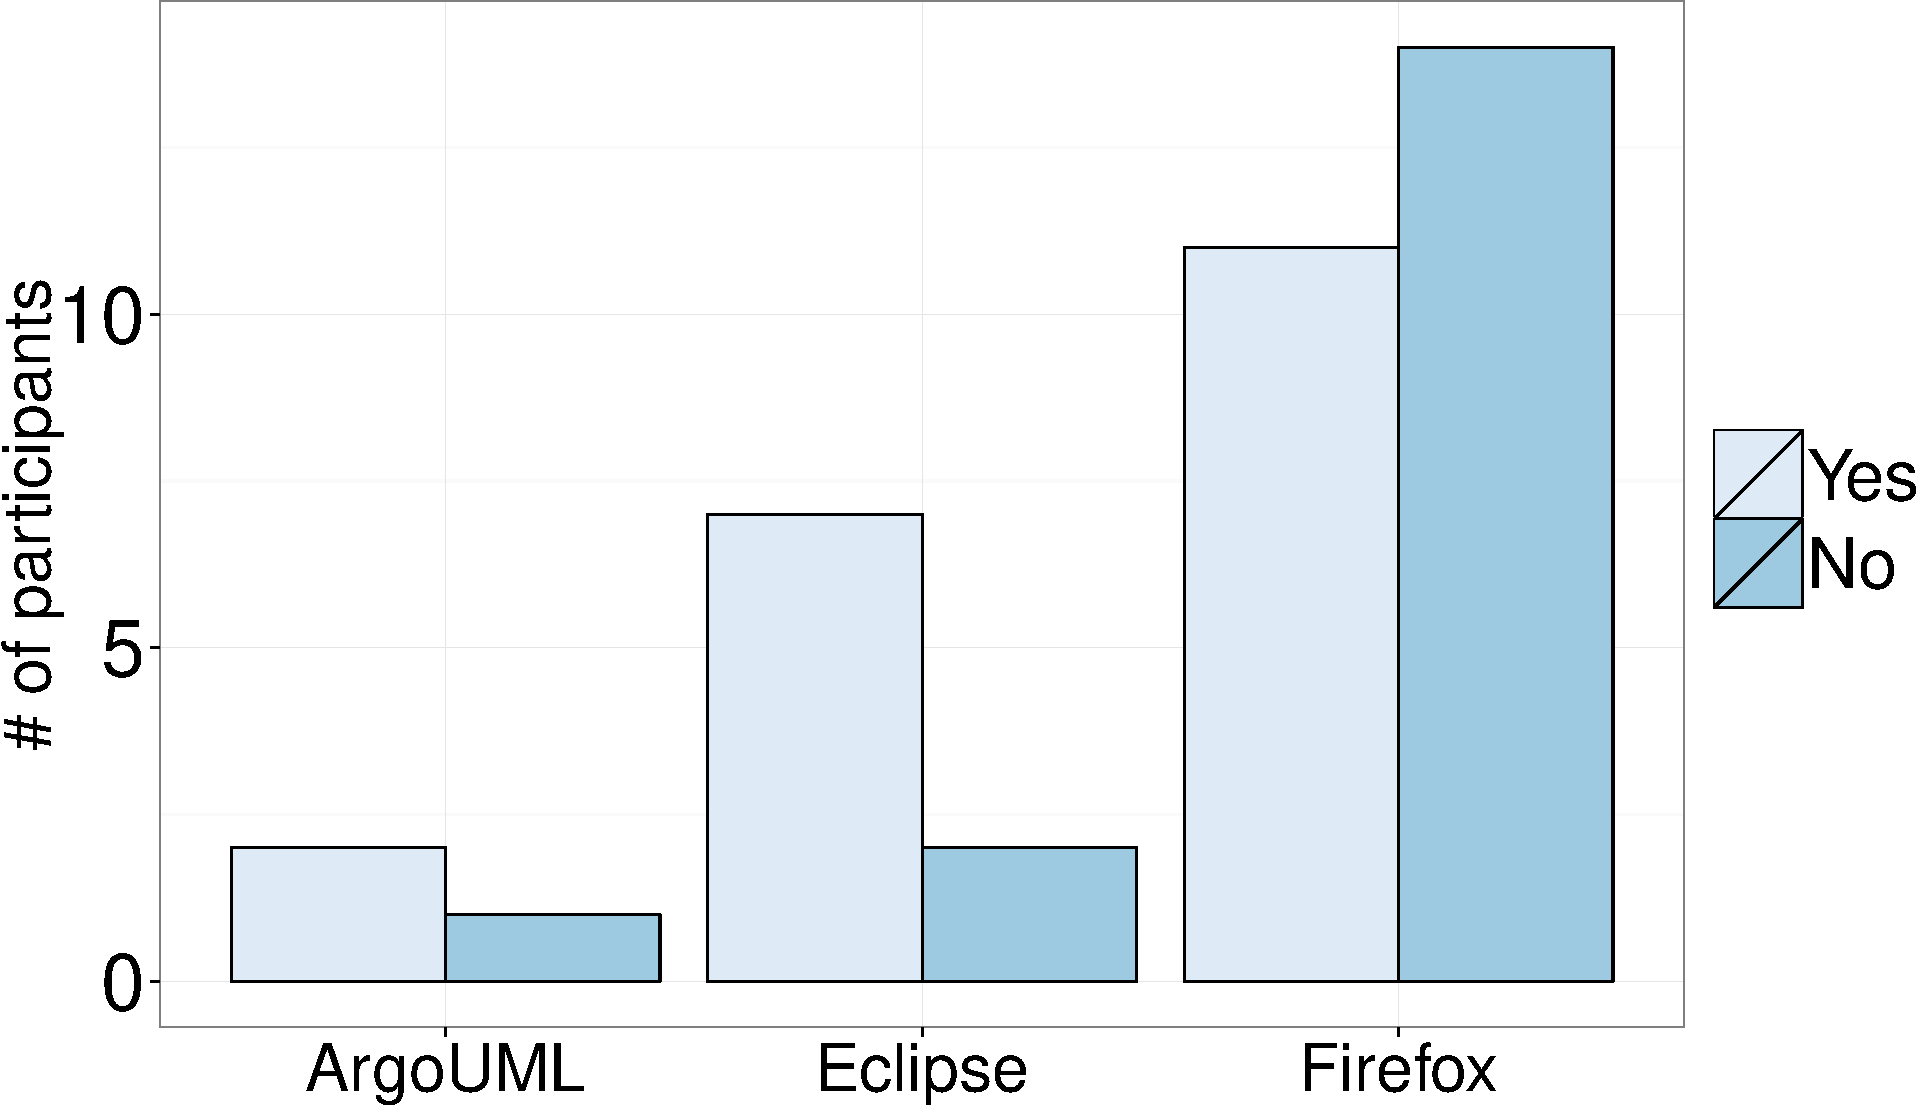
\includegraphics[width=0.80\textwidth,keepaspectratio] 
	{chapters/chapter5/figures/demographic_rapid_releases.pdf}
	\caption{Experience of the participants with respect to rapid release
	cycles.}
	\label{fig:demographics_rapid_releases}
\end{figure}
Moreover,
\hyperref[fig:demographics_rapid_releases]{Figure}~\ref{fig:demographics_rapid_releases}
shows how many participants have experience in working on rapid release cycles
({\em question~\#14}). We note that 57\% ($\frac{21}{37}$) of the participants
have some experience with rapid release cycles.
\begin{figure}
	\centering
	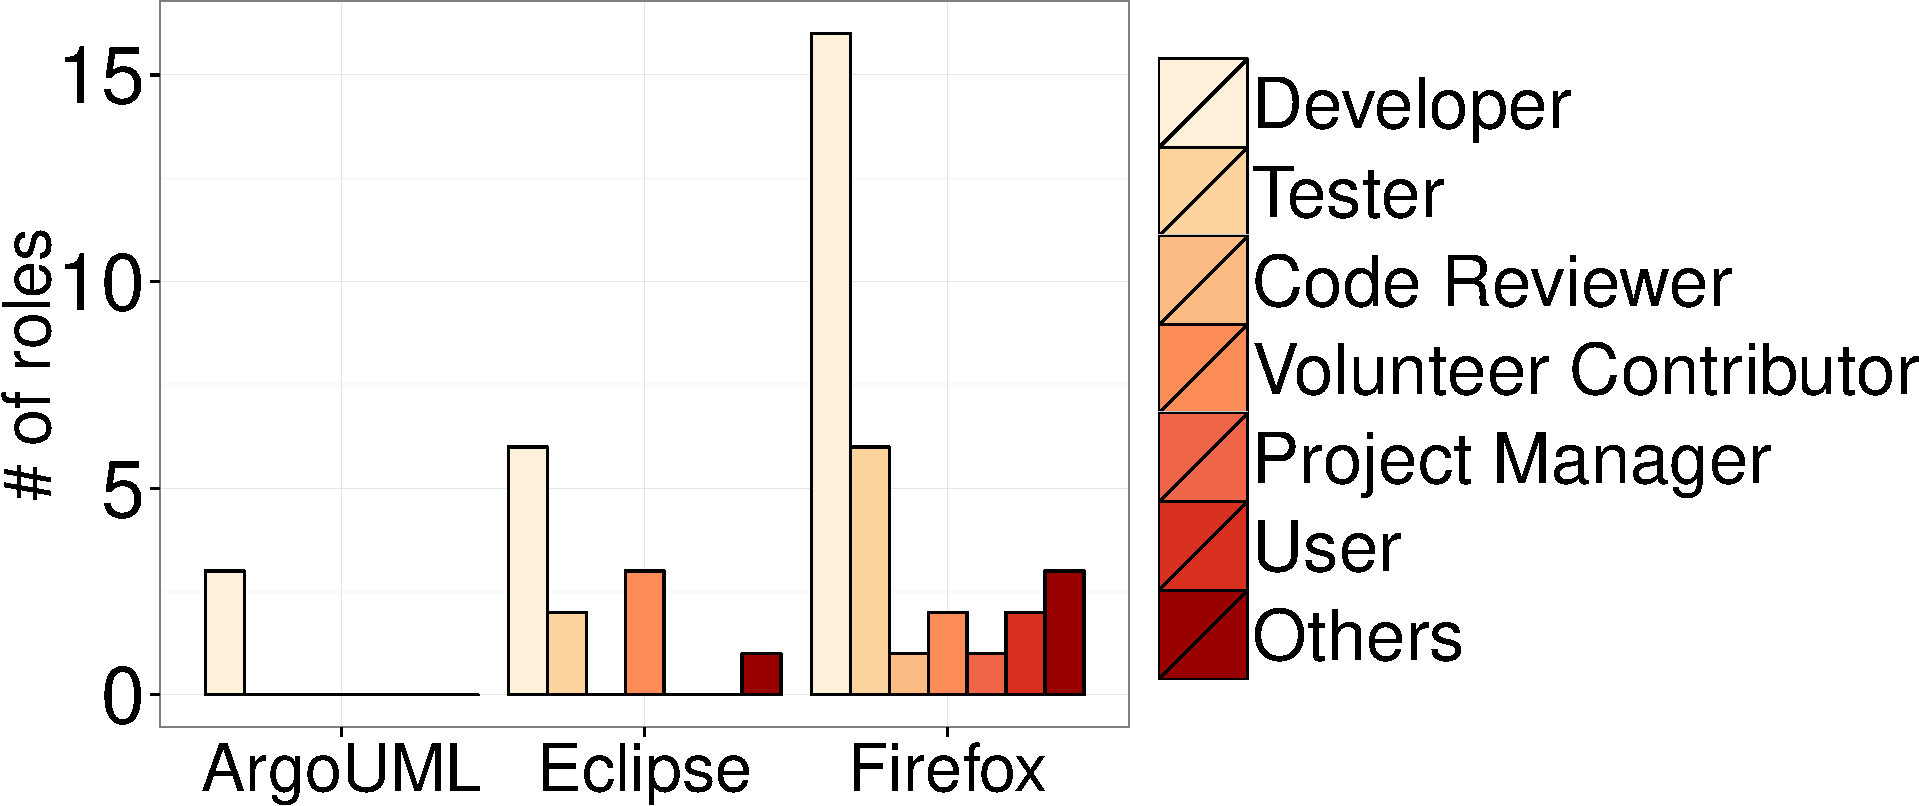
\includegraphics[width=0.80\textwidth,keepaspectratio] 
	{chapters/chapter5/figures/roles_demographics.pdf}
	\caption{An overview of the roles of the participants. One participant
	may have more than one role.}
	\label{fig:roles_demographics}
\end{figure}
\hyperref[fig:roles_demographics]{Figure}~\ref{fig:roles_demographics} shows the
team roles that the participants classified themselves as ({\em question~\#3}).
The majority of the participants consider themselves as ``developers'' and
``testers''. Since one participant can occupy several roles, the numbers that
are shown in
\hyperref[fig:roles_demographics]{Figure}~\ref{fig:roles_demographics} represent
the frequency that a role was cited rather than the number of participants.
\begin{figure}
	\centering
	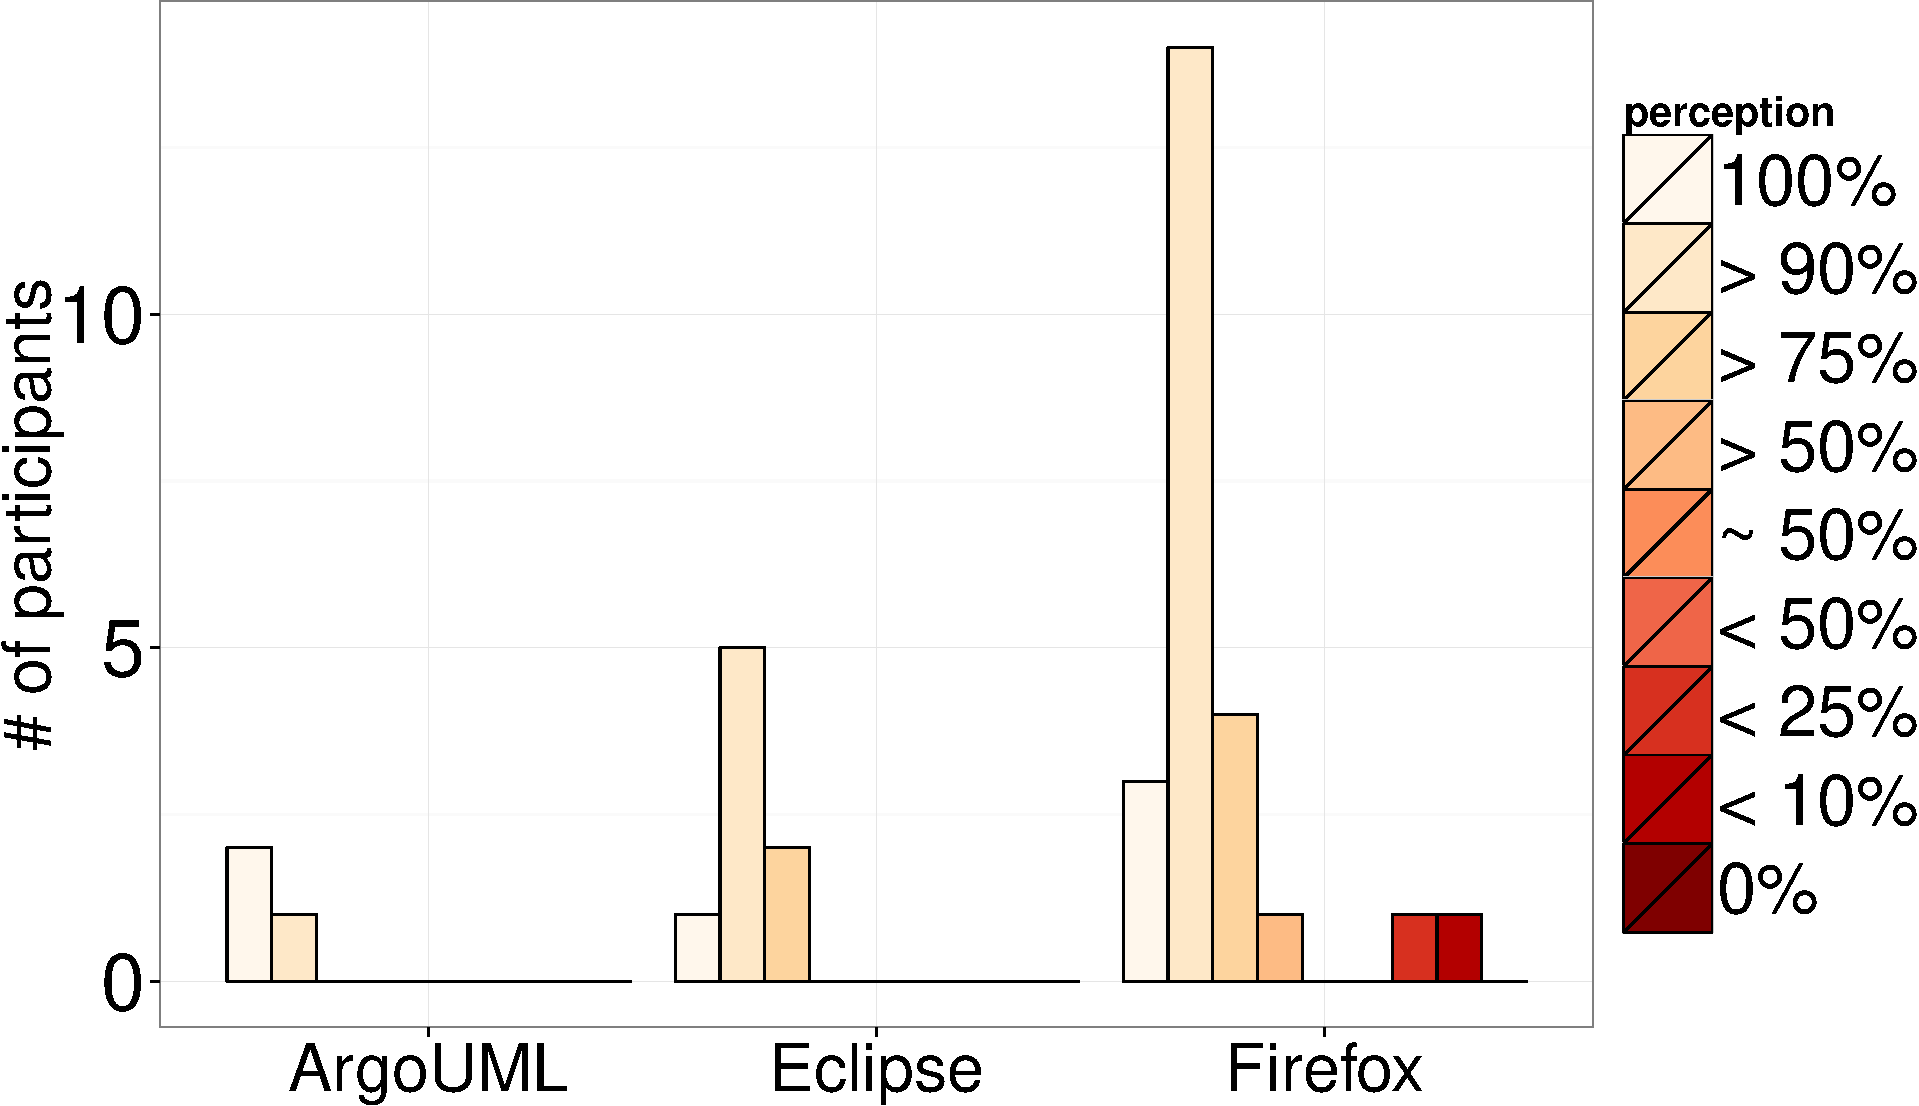
\includegraphics[width=0.80\textwidth,keepaspectratio] 
	{chapters/chapter5/figures/delay_perception.pdf}
	\caption{Participants' perception on how frequent is delivery delay. The data is grouped by proportions of
		how many addressed issues are included in the next possible
		release. This data refers to the responses to {\em question~\#6}.}
	\label{fig:delay_perception}
\end{figure}
Finally, we observe that the majority of the participants perceive delivery
delay as an unusual event rather than typical (see
\hyperref[fig:delay_perception]{Figure}~\ref{fig:delay_perception}). For
instance, 14 of the Firefox participants think that 90\% of the issues are
included in the next possible release.

In our analyses to answer \hyperref[ch5:rq1]{RQ1}-\hyperref[ch5:rq3]{RQ3}, we
attempt to correlate the rating of factors that are provided in {\em
question~\#13} with the data that is presented in this preliminary analysis.

\section{Results} \label{ch6:results}

We present the motivation, approach and obtained results for each investigated
RQ below.

\subsection{RQ1: What are developers' perceptions as to why delivery delays
occur?}\label{ch5:rq1}

\subsubsection*{RQ1: Motivation}

To the best of our knowledge, there is no prior work that qualitatively studies
delivery delay. Qualitative studies are important to detect phenomena that are
difficult to uncover quantitatively. Our goal in this RQ is to better understand
{\em \underline{why}} delivery delays happen. This investigation is a starting
point to reveal new ways of mitigating delivery delays.\\

\subsubsection*{RQ1: Results}

\begin{sloppypar} Our findings about developers' perceptions of the causes of
	delivery delay is divided into the following themes: {\em (i)
	development activities}, {\em (ii) decision making}, {\em (iii) risk},
	and {\em (iv) team collaboration}. Also, we observe that {\em (v)
	frustration} is a main perceived consequence of delivery delays. After
	discussing each theme below, we present a quantitative analysis of the
	factors that can impact delivery delay using the responses to {\em
	question~\#13} (see our \hyperref[ch5:datacollection2]{data collection}
	process).\\ 

\noindent\finding{Development activities.}{find25} 
The number of tests that should be executed was a recurrent theme among
participants. For instance, several participants stated that {\em additional
testing}$^{(12)}$ should be executed in order to avoid delivery delay. {\em
F17} states that the lack of {\em ``actual user testing beyond what QA can
provide''} can lead to delivery delay. Additionally, according to {\em F15},
{\em ``the most common reason is that testing was incomplete''} and according to {\em
F19}, delivery delay may happen because {\em ``testing has been too
narrow''.} Finally, {\em E32} voices concerns about integration testing: {\em
``No integration tests has been done.''} Such observations bring us back to a
core software engineering problem of when is testing
sufficient?~\cite{beller2015much,alghamdi2016automated}.

Other recurrent themes that emerged during our qualitative analysis are {\em
workload}$^{(7)}$ and {\em code review}.$^{(7)}$ For example, {\em E30} states
that {\em ``As the delayed completed issues stack up, they are harder to
integrate (the codebase is constantly changing, merge issues might emerge).''}
Interestingly, our statistical models in our prior work (see
\hyperref[ch:study12]{Chapter}~\ref{ch:study12})
indicate {\em workload}$^{(7)}$ as a metric that shares a strong relationship
with delivery delay. As for {\em code review},$^{(7)}$ the {\em
``Unavailability of the lead/reviewer/[Project Management Committee] (PMC)''} is
a reason of delivery delay that is pointed out by {\em E26}, while {\em F08}
argues that a {\em ``prompt code reviews [may] help''} to avoid delivery
delays~\cite{mcintosh2016emse}.\\

\noindent\finding{Decision making.}{find26} Decision making refers to the
activities that are not directly related to software construction, but can
influence the speed at which software is shipped. For example, how early a
codebase should be ``frozen''? Which issues should be prioritized? The {\em
timing}$^{(9)}$ and {\em prioritization}$^{(9)}$ are the recurrent themes in
our survey responses. For instance, two of the participants stated that issues
can be delayed because they are addressed {\em ``too late in the release
cycle''} ({\em E28}) or because they were addressed in a {\em ``long release
cycle.''} Also, {\em F12}'s opinion about how to avoid delivery delay is to
{\em ``test [addressed issues] early using real users (\eg on the pre-release
channels).''} Regarding {\em prioritization},$^{(9)}$ {\em E28} argues that team
members should {\em ``try to complete most important things early in the release
cycle''} to avoid delivery delay. Additionally, {\em F07} points out how
re-prioritization of issues is important: {\em ``[...] prioritizing and
re-prioritizing tasks to be sure you are building things on time [...].''}\\

\noindent\finding{Risk.}{find27} The risk that is associated with shipping
addressed issues may generate delivery delay according to our participants.
Among the risky addressed issues, the ones that have {\em
compatibility}$^{(12)}$ concerns are the most recurrent in this theme. For
example, when asked about reasons that may lead to delivery delay, {\em F12}
calls attention to issues that {\em ``break third-party websites''} and that can
generate {\em ``incompatibility with third-party software that users install.''}
Another risk that is associated with delivery delay is {\em stability}.$^{(9)}$
For instance, {\em F03} states that {\em ``when there are regressions noticed
during Aurora/Beta cycles,''} an addressed issue will likely skip the upcoming
official release.\\

\noindent\finding{Collaboration with other teams.}{find28}
Delivery delay may also occur due to
the overhead that is introduced when {\em collaboration}$^{(10)}$ is needed
between teams. For example, when asked to recall a delayed addressed
issue, {\em F23} answers that {\em ``sometimes, issues that require cross-team
cooperation may be delayed when the issue is differently prioritized by each
team.''} The {\em marketing}$^{(5)}$ team is mentioned recurrently when
delivery delay occurs due to other teams' collaboration. For instance,
according to {\em F21}, delivery delay {\em ``generally happens when
marketing wants to make a splash.''} {\em F08} also corroborates  {\em F21} by
stating that {\em ``product management [may] change their mind about the
desirability of a feature, or would like to time the release of the feature with
certain external events for marketing reasons.''}\\

\noindent\finding{Frustration.}{find29} Delivery delay may generate
frustration to both users and developers of the software. The majority of users'
frustration comes from their {\em expectation}$^{(20)}$ about the addressed
issues. {\em F07} makes an interesting analogy to explain user frustration: {\em
``as a user, it's like when you are waiting your suitcase in the airport to
come out on the belt. You know it has to be there, but you keep waiting.''}
{\em F14} also provides another analogy: {\em ``it's like a gift for Christmas,
but the day of Christmas is postponed.''} On the other hand, developers may get
frustrated for other reasons than users. The greatest frustration source for
developers is the feeling of {\em useless/unreleased work}.$^{(9)}$ According to
{\em F09}, when an addressed issue is delayed, a developer {\em ``feels like
[their] work is meaningless.''} {\em F04} complements {\em F09} by stating that
{\em ``it is frustrating to work on something and not see it shipped.''} \\

\noindent\finding{The time at which an issue is addressed
during a release cycle and the issue severity are the factors that receive the
highest ratings of importance.}{find30} In {\em
question~\#13} of our survey, we ask participants to rate the degree to which a
factor is related to delivery delay. The factors that we list are: the
reporter, the resolver, the priority, the severity, the number of comments, the
number of modified files, the number of modified LOC, and the time at which an
issue was addressed during a release cycle. The responses to {\em question~\#13}
are based on a 5-points-Likert scale, \ie participants rate factors using ranks from 1
(strongly disagree) to 5 (strongly agree). 

\begin{figure}
	\centering
	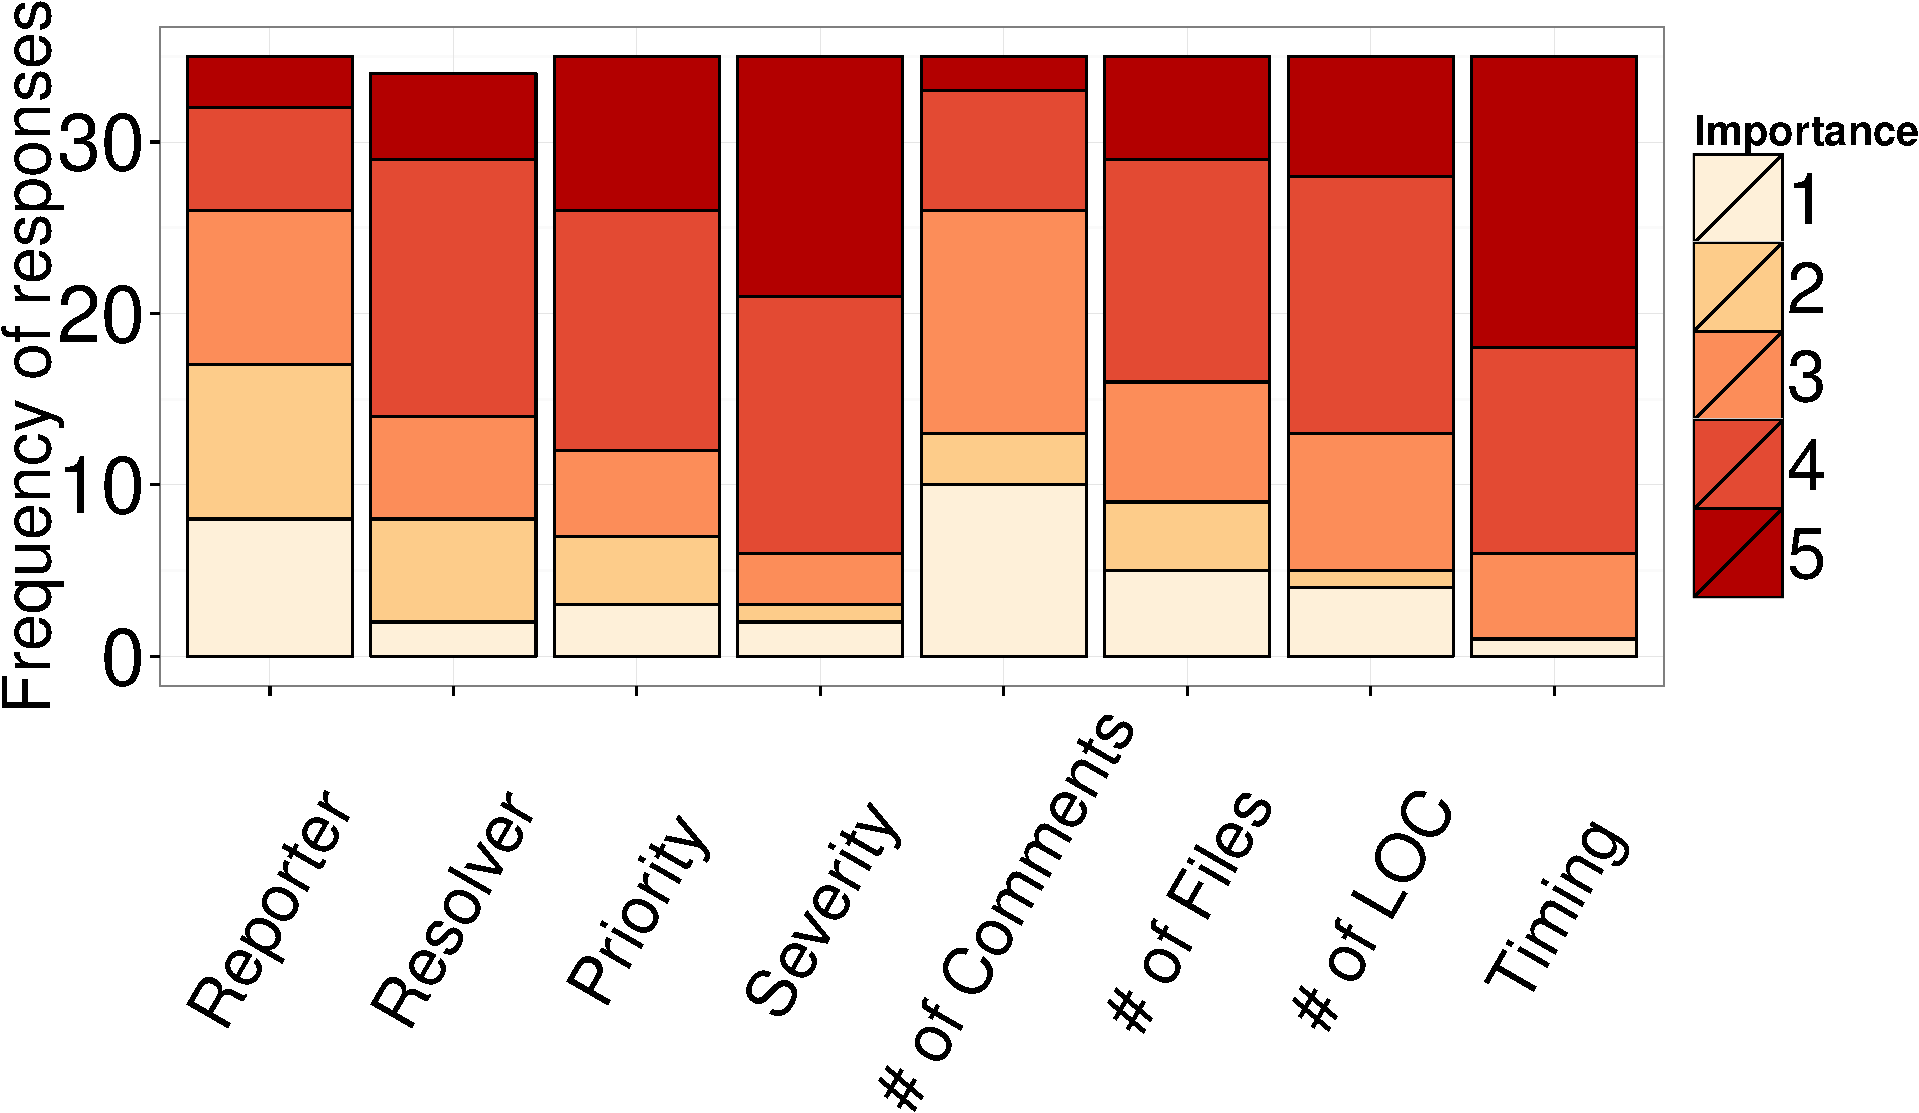
\includegraphics[width=0.80\textwidth,keepaspectratio]
	{chapters/chapter5/figures/rank_frequency.pdf}
	\caption{Frequency of ranks per factor.}
	\label{fig:rank_frequency}
\end{figure}

\begin{table}
	\footnotesize
	\centering
	\caption{Rating of factors related to delivery delay. The highest
		ratings are in bold.
		\label{tbl:factors}
	}
	\begin{tabular}{lr}
		\hline 
		\textbf{Factor} & \textbf{Average rating (mean)}\tabularnewline
		\hline 
		\hline 
		Time at which an issue is addressed during a release cycle (timing) & \textbf{4.257}\tabularnewline
		\hline 
		Severity & \textbf{4.086}\tabularnewline
		\hline 
		Priority & 3.629\tabularnewline
		\hline 
		Number of LOC & 3.571\tabularnewline
		\hline 
		Resolver & 3.441\tabularnewline
		\hline 
		Number of files & 3.314\tabularnewline
		\hline 
		Number of comments & 2.657\tabularnewline
		\hline 
		Reporter & 2.629\tabularnewline
		\hline 
	\end{tabular}
\end{table}

In \hyperref[fig:rank_frequency]{Figure}~\ref{fig:rank_frequency}, we show the
frequency of each rank per factor, while we show the average rating of each
factor in \hyperref[tbl:factors]{Table}~\ref{tbl:factors}. We observe that the
factors that receive the highest ranks are {\em severity} and {\em timing}.
Regarding {\em timing}, this result is in agreement with our regression models
that are presented in RQ3, in which {\em cycle queue rank} is one of the most
influential variables (see \hyperref[find22]{Finding}~\ref{find22}). Indeed,
during the interview, {\em F06} further explains that if an issue that is risky
is addressed in the end of a release cycle, such an issue is likely to be
delayed to the next cycle, so that it can receive additional testing. However,
the importance ranks that were assigned to the {\em severity} factor contradicts
what we observed in our statistical models (see
\hyperref[find11]{Finding}~\ref{find11}). During another interview, participant
{\em F23} explains that the high importance rating that was given to the {\em
severity} factor is due to the real severity of an issue---not the severity
value that is often assigned in issue reports. In fact, the study that was
conducted by Herraiz~\etal hints that the severity field of an issue report may
be inaccurate~\cite{Herraiz2008}.

\begin{figure}
	\centering
	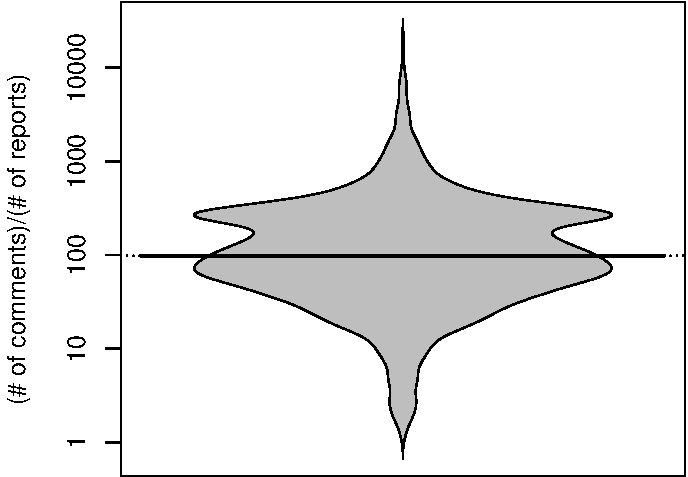
\includegraphics[width=.8\textwidth,keepaspectratio]
	{chapters/chapter5/figures/comments_ratio.pdf}
	\caption{Distribution of number of comments normalized by the number of
	reported issues.}
	\label{fig:comments_ratio}
\end{figure}

On the other hand, the factors with the lowest ranks are {\em reporter}, and
{\em \# of comments}. We also asked our interviewees about these lower ratings.
One of our interviewees explained that the reporter of an issue might influence
delivery delay only in cases in which the reporter is also a Firefox employee.
In these cases, the reporter will address the issue her/himself, which can speed
up the shipping process.\smartfoot{We did not observe a statistically
	significant difference in delivery delays between issues that are
addressed by the reporters themselves and issues that are addressed by a
different team member.} As for the {\em \# of comments}, another interviewee
clarified that there are several passionate people on bugs that can inflate the
number of comments even if the issue is easy to ship. For each reporter, we
normalize the number of his/her comments by the number of his/her reported
issues.  We plot the distribution of the normalized number of comments in
\hyperref[fig:comments_ratio]{Figure}~\ref{fig:comments_ratio}. The median
number of comments per reported issue is 98. Indeed, we observe reporters with a
great number of comments (\eg 500 to 10,000 comments) per reported issue.  This
result suggest that the perception of our interviewee is likely to be true.

\begin{table}
	\scriptsize
	\centering
	\caption{$P$-$values$ of the comparisons between factors. Values in bold are $<$ 0.05.
		\label{tbl:pvalues_factors}
	}
	\begin{tabular}{lrrrr}
		\hline 
		Factor x Factor & Reporter & Resolver & Priority & Severity\tabularnewline
		\hline 
		\hline 
		Reporter & --- & 1.2$e^{-1}$ & \textbf{1.3$e^{-2}$} & \textbf{1.4$e^{-5}$} \tabularnewline
		\hline 
		Resolver & 1.2$e^{-1}$ & --- & 1 & 1.2$e^{-1}$ \tabularnewline
		\hline 
		Priority & \textbf{1.3$e^{-2}$} & \textbf{1.3$e^{-2}$} & --- & 4.8$e^{-1}$ \tabularnewline
		\hline 
		Severity & \textbf{1.4$e^{-5}$} & 1.2$e^{-1}$ & 4.7$e^{-1}$ & ---\tabularnewline
		\hline 
		\# of Comments & 4.8$e^{-1}$ & 1.2$e^{-1}$ & \textbf{1.4$e^{-2}$} & \textbf{1.6$e^{-5}$} \tabularnewline
		\hline 
		\# of Files & 1.8$e^{-1}$ & 7.9$e^{-1}$ & 1 & 6.6$e^{-2}$ \tabularnewline
		\hline 
		\# of LOC & \textbf{3.0$e^{-2}$} & 1 & 1 & 2.8$e^{-1}$ \tabularnewline
		\hline 
		Timing & \textbf{8.0$e^{-7}$} & \textbf{3.2$e^{-2}$} & 1.8$e^{-1}$ & 1\tabularnewline
		\hline 
		\hline
		Factor x Factor & \# of Comments & \# of Files & \# of LOC & Timing\tabularnewline
		\hline 
		Reporter & 4.8$e^{-1}$ & 1.8$e^{-1}$ & \textbf{3.0$e^{-2}$} & \textbf{8.1$e^{-7}$} \tabularnewline
		\hline 
		Resolver & 1.2$e^{-1}$ & 7.9$e^{-1}$ & 1 & \textbf{3.2$e^{-2}$} \tabularnewline
		\hline 
		Priority & \textbf{1.4$e^{-2}$} & 1 & 1 & 1.8$e^{-1}$ \tabularnewline
		\hline 
		Severity & \textbf{1.6$e^{-5}$} & 6.6$e^{-2}$ & 2.8$e^{-1}$ & 1\tabularnewline
		\hline 
		\# of Comments & --- & 1.7$e^{-1}$ & \textbf{3.3$e^{-2}$} & \textbf{9.6$e^{-7}$} \tabularnewline
		\hline 
		\# of Files & 1.7$e^{-1}$ & --- & 1 & \textbf{1.4$e^{-2}$} \tabularnewline
		\hline 
		\# of LOC & 3.3$e^{-2}$ & 1 & --- & 1.1$e^{-1}$ \tabularnewline
		\hline 
		Timing & \textbf{9.6$e^{-7}$} & \textbf{1.4$e^{-2}$} & 1.1$e^{-1}$ & ---\tabularnewline
		\hline 
	\end{tabular}
\end{table}

A Kruskal Wallis test indicates that the difference in ratings between metrics
are statistically significant ($p=0.01507$).
\hyperref[tbl:pvalues_factors]{Table}~\ref{tbl:pvalues_factors} shows the
Bonferroni corrected $p$-$values$ of the Dunn tests. We observe that the {\em
timing} factor has significant larger response values than all the other factors except
the {\em severity}, {\em priority}, and {\em LOC} factors ($p<0.05$).

We also use Spearman's $\rho$ to correlate the rating of the factors with (i)
general experience ({\em question \#1}) and (ii) project experience ({\em
question \#2}). The only statistically significant correlation that we observe is
between the {\em timing} factor and general experience. We achieve a negative
correlation of -0.36 ($p=0.03235$). This result suggests that less
experienced participants tend to report that the time at which an issue is
addressed during a release cycle plays a more important role in delivery
delay. One of our interviewees explains this observation by stating that {\em
``when an issue is addressed early in the release cycle, it should have more
time to be tested before integration,''} which can be helpful for fixes
from less experienced resolvers. Finally, we also correlate the responses
to {\em question~\#6} with general and project experience. However, no
significant correlations were found.\\
\end{sloppypar}

\conclusionbox{Our survey participants report that the delivery of addressed
issues may be delayed due to reasons that are related to the development
activities, decision making, team collaboration, or risk. Moreover, delivery
delay likely lead to user/developer frustration.}

\subsection{RQ2: What are the perceived impacts of rapid
releases on delivery delays?}\label{ch5:rq2}

\subsubsection*{RQ2: Motivation}

In this research question, we intend to complement our quantitative findings
about the comparison between traditional and rapid release cycles regarding
delivery delays. This investigation is important to gain deeper explanations as
to why addressed issues may be delivered more quickly in traditional releases.
Additionally, we intend to understand what are the reasons for the perceived
success of adopting a rapid release cycle. This is also important to help
project leaders with their decision of adopting a rapid release cycle rather
than a traditional one. \\

\subsubsection*{RQ2: Results}

In this RQ, we study the perceptions of developers about the impact of shifting
to a rapid release cycle with respect to delivery delays. Our findings about
these perceptions are organized along the following themes: {\em management},
{\em delivery}, and {\em development}. We describe each theme below.\\    

\noindent\finding{Management.}{find31} The shift to a rapid
release cycle has a considerable impact on release cycle management. 

The most recurrent theme in this respect is {\em flexibility}$^{(4)}$ to plan
the scope of the releases that should be shipped.  {\em F01}'s opinion is that
rapid releases {\em ``provide a bit more flexibility, since if an important
issue pushed back a less important change and it misses the release cycle, it's
not a huge deal with rapid releases.''} {\em F01}'s observation is supported by
our finding that rapid Firefox releases tend to deliver addressed issues
more consistently (see \hyperref[find18]{Finding}~\ref{find18}). 

Another perceived advantage of rapid release cycles are the {\em risk
mitigation}$^{(3)}$ and {\em better prioritization}.$^{(3)}$ With respect to
{\em risk mitigation},$^{(3)}$ {\em F07} argues that in rapid release cycles,
the team is {\em ``able to identify issues sooner. It is easier to identify
issues when you have only deployed 3 new commits than 100.''} As for {\em better
prioritization},$^{(3)}$ {\em F19} explains that rapid release cycles {\em
``probably decreases unnecessary delays of the releases because deadline is
closer and developers have to react faster for the pressuring issues.
Non-critical issues gets also pushed back and don't receive useless attention
nor create delays.''} Still on the {\em better prioritization}$^{(3)}$ matter,
{\em F17} adds that rapid releases {\em ``provide a time box in which [the team]
must forecast the top priority work to complete within that time frame.'' }\\

\noindent\finding{Delivery.}{find32} The most recurrent perceived
advantage of rapid release cycles is the {\em ``faster delivery''}$^{(33)}$
of new functionalities. When asked about the motivation to use rapid release
cycles, {\em F05} mentions {\em ``increasing speed of getting new features to
users,''} while {\em F06} mentions a similar statement: {\em ``getting new features to
users sooner.''} Interestingly, not all participants that mentioned the time to
deliver new functionalities report that rapid releases always reduce such time.
For {\em F22}, rapid releases {\em ``reduce the time to deliver issues to end
users in some cases, and lengthen them in others.''} More specifically, {\em F24} 
says that {\em ``Low priority issues (new features) take less
time to be delivered, whereas high priority ones (important bugs) take more
time.''} 

Another recurrent perception about rapid releases is the {\em faster user
feedback}$^{(17)}$ due to the constant delivery of new functionalities. For
instance, {\em E29} provides an example that {\em ``you don't find yourself
fixing a bug that you introduced two years ago which the field only discovered on the
release.''}\\

\noindent\finding{Development.}{find33}
We do not observe a specific theme that is recurrent with respect
to development activities. Instead, we observe a broad range of themes that are
cited by the participants. Among such themes, we observe {\em quality},$^{(3)}$
{\em more functionalities},$^{(2)}$ {\em better motivation},$^{(2)}$ and {\em
better prototyping}.$^{(2)}$ Quality should be a measure of success of using
rapid release cycles. According to {\em E26}, {\em ``quality of delivered code
should remain the same or improve''} after switching to rapid releases. Another
way to measure the success of a rapid release cycle is the {\em number of
functionalities}$^{(2)}$ that are completed. {\em E34} states the following: {\em
``I would see if more issues were completely fixed''} as a measure of success. 

Moreover, rapid releases may also impact team members' motivation. For instance,
{\em F06}'s opinion about why to switch to rapid release cycles is {\em ``the
need to motivate the community via more frequent collaboration.''} Finally,
rapid release cycles may also improve prototyping activities. For instance, {\em
E27} argues that, by adopting rapid releases, a development team can {\em ``fix
bugs quickly [and] prototype features, having results in few months.''}

\conclusionbox{The allure of delivering addressed
issues more quickly to users is the most recurrent motivator of switching to a
rapid release cycle. Moreover, the allure of improving management flexibility and quality
of addressed issues are other advantages that are perceived by our participants
with respect to switching to rapid release cycles.}

\subsection{RQ3: Do participants agree with our quantitative
findings about delivery delay?}\label{ch5:rq3}

\subsubsection*{RQ3: Motivation}

The main motivation for this research question is to solicit feedback about our
quantitative findings. More specifically, we aim to understand whether our
quantitative findings resonates with the participants' perception of delivery
delays.

\subsubsection*{RQ3: Results}

In this research question, we investigate how our participants feel about the
data that we collect during our prior quantitative studies
(\hyperref[st:study1]{Studies}~\ref{st:study1} and~\ref{st:study3}). This
research question is divided into two subsections---one for each {\em theme}
that is investigated in this thesis---{\em (i)} reasons for delivery delay in
general and {\em (ii)} the impact of rapid release cycles on delivery delay
(\hyperref[fig:thesis_overview]{Figure}~\ref{fig:thesis_overview}).\\

\noindent\finding{delivery delay in general.}{find34}
In this analysis, we present the data that we collect in our prior studies
(\hyperref[ch:study12]{Chapter}~\ref{ch:study12}) and investigate if this data
resonates with participants' experience. We provide the methodology of our
data-related questions to participants through a web page that is mentioned in
our surveys (see~\hyperref[methodology:i]{Appendix}~\ref{methodology:i}).

\begin{figure}
	\centering
	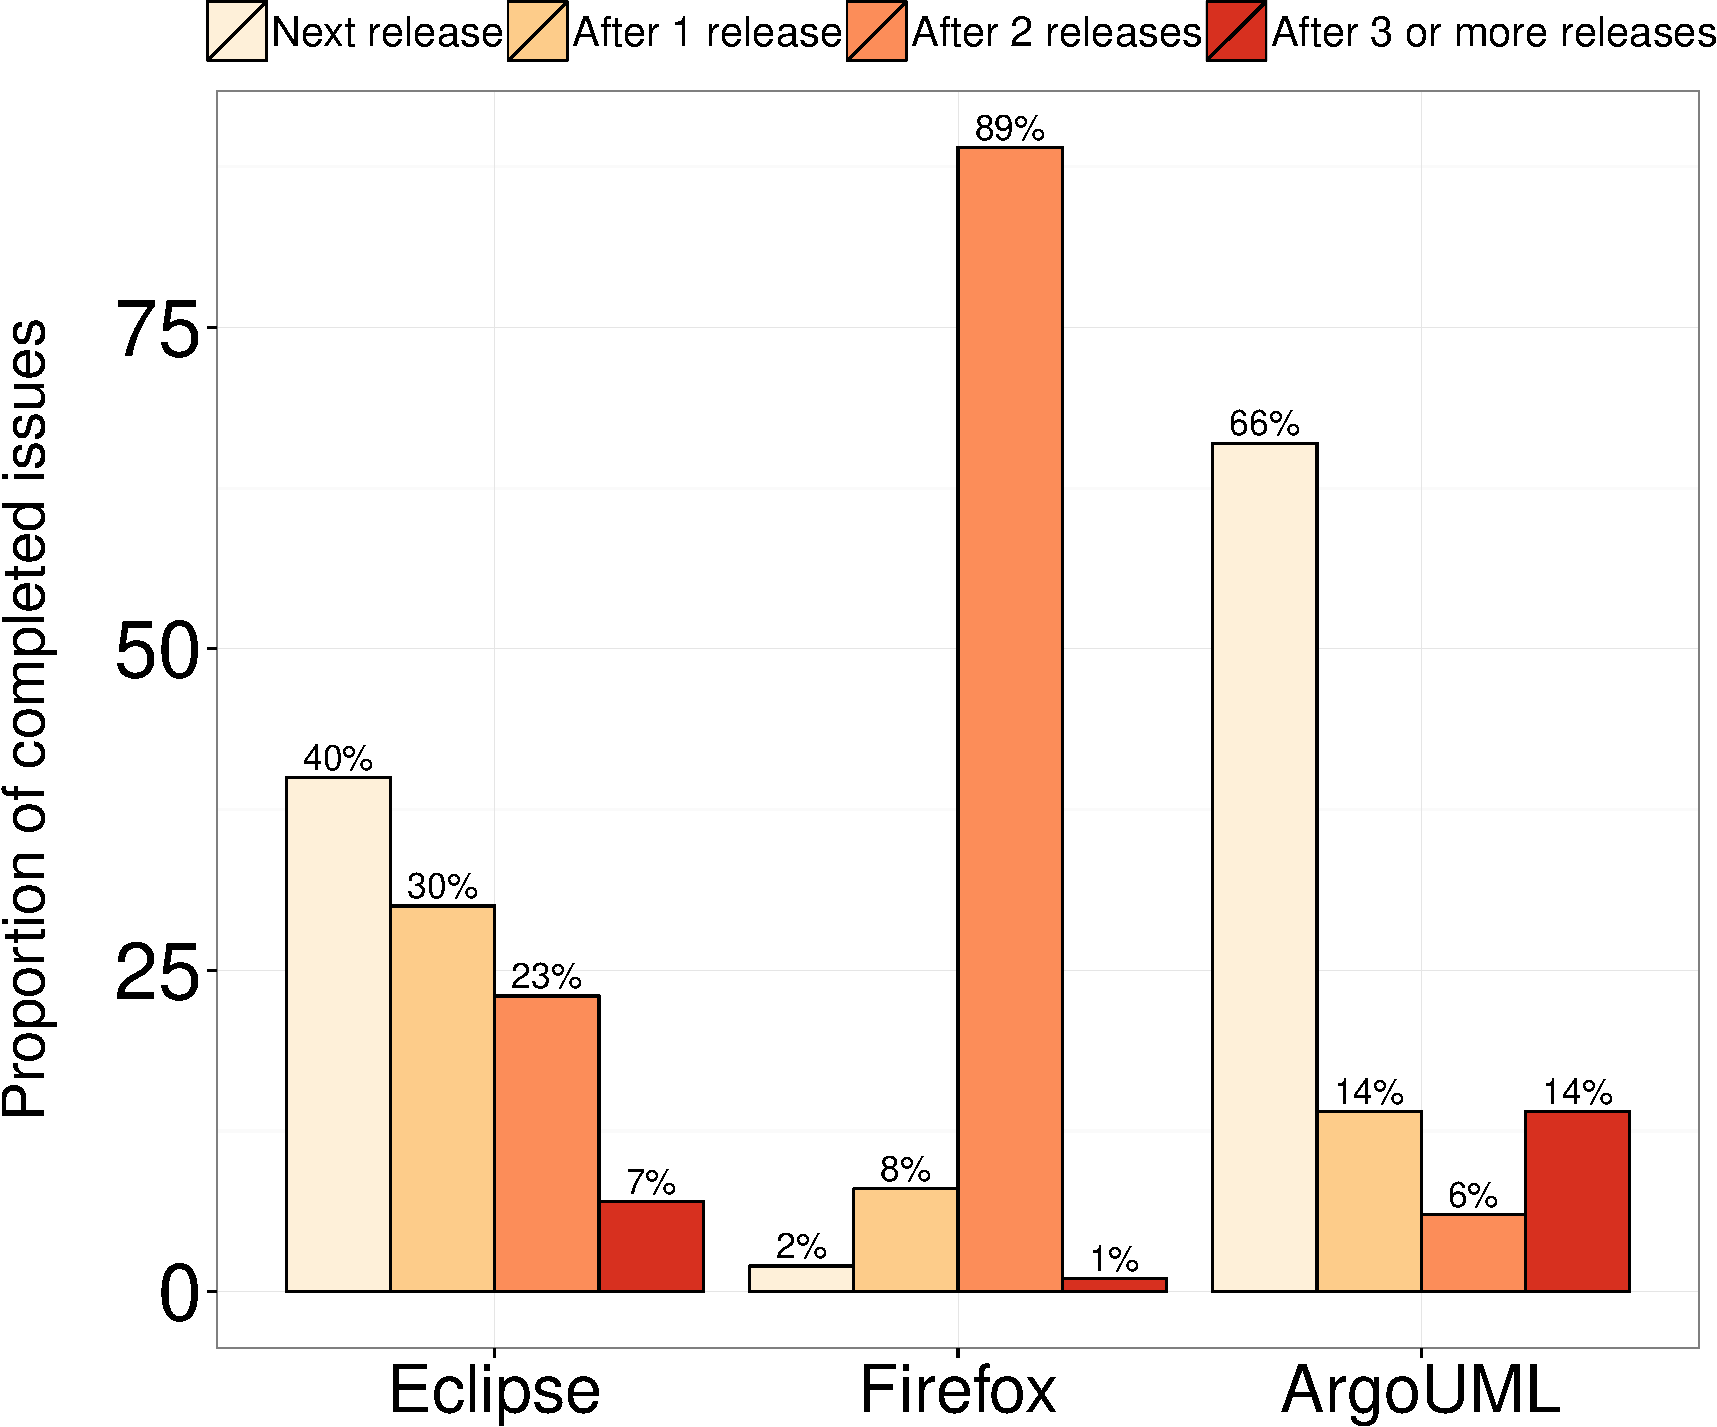
\includegraphics[width=0.80\textwidth,keepaspectratio]
	{chapters/chapter4/figures/CS_rq1-datasets.pdf}
	\caption{Proportion of addressed issues that have their delivery
		delayed by a given number of releases. For example, 89\% of the
	addressed issues skip two Firefox stable releases before being shipped
to users (this chart was already presented in
\hyperref[ch:study12]{Chapter}~\ref{ch:study12}. }
	\label{fig:data-related-rq1}
\end{figure}

\hyperref[fig:data-related-rq1]{Figure}~\ref{fig:data-related-rq1} shows the
chart that we presented to participants. For example, 89\% of the addressed
issues skip two Firefox stable releases before being shipped to users. The most
recurrent themes among the responses of participants to explain this data are:
{\em team workload}$^{(5)}$ and {\em dependency}.$^{(2)}$ Among the responses
that are related to {\em team workload},$^{(5)}$ {\em E27} explains that {\em
``committers  are too busy,''} while {\em E26} argues that there might be {\em
``delay[s] in review[s] when the issues [are] completed,''} which can generate
delivery delay. Regarding {\em dependency},$^{(2)}$ {\em E32}'s opinion is that
delivery delay may happen due to {\em ``the strong connection to other Eclipse
projects which makes integration more costly (time consuming).''} Furthermore,
two of our interviewees ({\em F11} and {\em F23}) provide us with examples of
why addressed issues may be delayed due to dependency problems. For example,
{\em F23} explains that delivery delay can happen when there are {\em
``dependencies between projects and one of them gets done, but the other
implementation takes a longer while.''} Another example, provided by {\em F23}
is when {\em ``you release a bug fix but then you realize: Hey! These users are
	not able to use these websites anymore because web servers implement the
	spec in a wrong way or do some really weird things that are not
expected.''}

Additionally, we ask participants from the Eclipse and ArgoUML projects about
their opinion regarding why the data from the Firefox project behaves differently from
theirs, \ie a larger number of releases being skipped by addressed issues. The
most recurrent responses explain that this difference may be due to the {\em
rapid release cycle}$^{(4)}$ that is adopted by the Firefox project. For
example, {\em E30}'s opinion is that {\em ``on a rapid release cycle
	(e.g. 6 weeks for firefox), a two-release delay means 12 weeks,
	less than 3 months, which is still less than no delay for a fix
submitted early in a project with a 6-month release cycle.''} 
\\           

\noindent\finding{Impact of switching to a rapid release cycle.}{find35}
We present the data that is shown in
\hyperref[fig:traditional_vs_rapid]{Figure}~\ref{fig:traditional_vs_rapid} to
the participants of the Firefox project.
\hyperref[fig:traditional_vs_rapid]{Figure}~\ref{fig:traditional_vs_rapid}
compares the delivery delay between traditional and rapid release cycles. We
then ask whether this result resonates with the participants' experience. More
details about how we show this data to participants can be found in
\hyperref[methodology:ii]{Appendix}~\ref{methodology:ii}. From the 14 responses
that we received for this question, 5 participants explicitly disagree with our
analysis, while 6 participants explicitly agree with it. 

We could interview only two participants that disagree with the results ({\em
F06} and {\em F09}). After providing extra explanation about our methodology and
asking them to elaborate on their responses, we could better understand their
reasons.  {\em F06} clarifies: {\em ``I'm not surprised that there are things in
that bucket''} (the short delays due to minor traditional releases), instead
{\em ``I'm surprised that there are many of them.''} In addition, {\em F09}
declared {\em ``I misunderstood [your] question, but now it [(the data)] makes
sense.''} With respect to the remaining participants that disagree with our
results, they inform us that the data does not resonate with their experience.
For instance, {\em F21} provides the following opinion {\em ``this does not
resonate with my experience. I find the traditional model is much much slower
than rapid release to get fixes in users hands.''} Unfortunately, we did not
have the opportunity to interview such participants to better understand why our
data do not reasontes with their experience.

From the set of participants that agree with our results, two of them explain
that the behaviour that is presented by the traditional release data is due to
the {\em integration rush}$^{(2)}$ that happens prior to shipping. {\em F15}'s
opinion is that {\em ``since missing a release cycle isn't a big deal, more
features are kept from being released until they're properly polished instead of
being rushed at the end of a long release cycle.''} {\em F22} also provides us
with a reasonable explanation when stating that our result {\em ``makes perfect
	sense as issues will, unless fast-tracked or held back, be released a
	set quantum of time after they are completed. This is dominated by the
	timing of the release schedule, not by the timing of the discovery or
fix.''}\\

\conclusionbox{The dependency of addressed issues on other projects and team
	workload are major perceived reasons to explain our findings about
	delivery delays. Moreover, participants are divided when explaining
	why traditional releases may have shorter delivery delays.
	Nevertheless, the fact that in rapid releases an integration rush is no
	longer needed and that additional time can be spent on polishing
	addressed issues emerge as main explanations as to why traditional
releases can have shorter delivery delays.}

